\chapter{Contributions}
\label{sec:contributions}
\fixme{All subsections need to be expanded and further clarified.}

\fixme{Time of text: past or present?}

In this section we will tie together the different publications made during the course of the PhD studies. We will focus on the general message of the publications in relation to the goal of the PhD. We remand to the full text of the individual publications in Appendices~ \ref{sec:firstcontribution}-\ref{sec:lastcontribution} for the full technical details.

\section{Outline and motivation}

\fixme{(Figure: Fields in which we need instant feedback on appearance: 3d printing, artist feedback, quality control, meat)}

As we discussed in Chapters~\ref{sec:background} and~\ref{sec:related}, many efforts have been put forward by the community towards interactive physically based rendering. We barely scratched the surface on reporting some of these techniques in Chapter~\ref{sec:related}. These techniques are becoming widely popular in recent years, mainly due to increased GPU computational power. 

We argue that there is a need in the industry for photorealistic accurate interactive rendering. In many fields, people need immediate feedback on on the aspect of the final product. Some examples include visual inspection of produced parts, preview of 3D printed objects, artistic iterations for movie scenes, and prediction of the outcomes of an industrial process. In all these applications, different requirements are set on how fast the rendering should be. For example, in quality inspection of a produced part, minutes can be acceptable. For artistic feedback in movie production, this may go down to a few seconds, depending on the number of necessary iterations. In  the real-time rendering of a game or a virtual reality application, this can go as low as an handful of milliseconds. Our contributions over the course of the PhD studies contribute in various parts of this wide spectrum of needs.

Regarding our contributions, Contribution~\ref{sec:juice} provides a first example on why we need both fast and accurate rendering, in the form predicting the appearance of  cloudy apple juice after production. In Contribution~\ref{sec:glass} we discuss on the definition of photorealistic rendering, and how good a rendering should be to allow accurate parameter estimation. Afterwards, we will discuss Contribution~\ref{sec:interactivedirsss} an interactive method expanding current techniques to improve physical accuracy for translucent materials. We will conclude with two applications at the other end of the spectrum, one (\ref{sec:srt}) leveraging recent innovations in interactive ray tracing to solve a widespread problem in real time graphics, temporal stability, and one (\ref{sec:vrbrdf}) leveraging physically based materials in a hard real time physically based application. 

\section{Defining photorealistic rendering}
\begin{figure}[t]
\centering
\begin{tabular}{@{}c@{}c@{}}
	 \includegraphics[width=0.4\columnwidth]{figures/teaser_render.png} &
	 \includegraphics[width=0.4\columnwidth]{figures/ref_img.jpg}  \\
	rendering & photograph \\
\end{tabular}
\caption{Cloudy apple juice photographed and rendered the appearance model from Contribution~\ref{sec:juice}. In the model, we inferred apple particle concentration (0.8 g/l) and apple storage period (4 days) to match the photograph.} %The red rectangle shows where we estimated RMSE in Table \ref{table:quant}.}
\label{fig:juicecomparison}
\end{figure}

Our first discussion point is in what is photorealistic rendering, and the distinction between \emph{physically based} and \emph{photorealistic} rendering. In the former, the emphasis is onto creating rendering models and techniques that are based on physical radiometric processes. In the latter, we put emphasis on \emph{validating} the models with real images (see Figure~\ref{fig:juicecomparison}). Our first contributions~\ref{sec:glass} and~\ref{sec:juice} set out to test the limits of physically based rendering. In our work, we initially set to test how much a rendering can get close to real images. 

These two investigations led to a number of interesting insight on physically based rendering. A first insight is that renderings and pictures can be compared, and actual physical quantities can be measured from them (See Figure~\ref{fig:glasscomparison}). In our first contribution~\ref{sec:juice}, we created a new appearance model to predict the appearance of cloudy apple juice. The models uses data from various sources to create the rendering of a glass of apple juice. In our proof of concept model, we have the concentration of apple juice and the number of days the apples were stored as inputs. By comparing pictures with renderings made using this parameters, we can estimate them for any glass of cloudy apple juice. In our endeavor, we identified a number of different challenges in comparing pictures and renderings, mostly related to the scene. Subtle changes in the scene can lead to big differences in direct comparisons, especially when the material influences its surroundings, such and in the case of cloudy apple juice. See the light caustic next to the glass in Figure~\ref{fig:juicecomparison}. In this initial proof of concept, we simply compared a selected patch to get a rough estimate of the parameters.

\begin{figure}
\begin{tabular}{@{}c@{}c@{}}
	 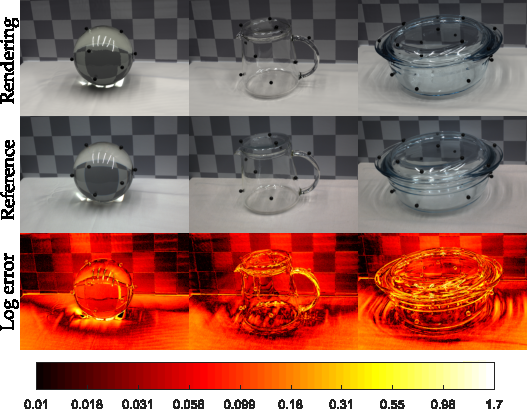
\includegraphics[height=4.3cm]{figures/comparison} & \hspace{2em}
	 \includegraphics[height=4.3cm]{figures/glass_bowl_analysis_by_synthesis}  \\
\end{tabular}
\caption{To the left, comparing quantitavely renderings (top row) with real images (mid row). Error is shown in the bottom row. On the right, estimating the absorption parameter $\sigma_a$ for the glass bowl. Each coefficient was estimated independently. Each dot in the graph corresponds to a rendered image. }
\label{fig:glasscomparison}
\end{figure}
In our main contribution~\ref{sec:glass}, we strive to improve upon the previous results of comparing rendering with images, for a different application. In this case, we are comparing images of glass objects, using a full pipeline to accurately estimate the scene, scan glass objects with CT scanners and placing them in the scene for final rendering. Our main contribution of this work is actually the pipeline, that allows researchers to compare pictures and renderings of glass objects, getting a quantitative comparison at the end. This will allow researchers to experiment with each step of the pipeline, improving upon the state of the art techniques used. As we can see from Figure~\ref{fig:glasscomparison} left, we are able to quantitatively compare images of glass objects with pictures, something that as never been done beforehand. At a first glance, the pictures and rendering are almost indistinguishable. This ability of qualitatively compare images and rendering would allow in the future to further improve existing techniques in acquisition, rendering and reconstruction. If the quality of the reconstruction becomes good enough, even path tracing could be compared with the original image. 

As in the previous contribution, absorbing glass is a material that greatly influences its surroundings, so material property estimation is not trivial. As in contribution~\ref{sec:juice}, we use the comparisons to measure material properties, in this case the index of refraction and the spectral absorption coefficient $\sigma_a$ of the glass objects, as we can see in Figure~\ref{fig:glasscomparison}, right. To estimate the material properties we need to generate many of them. Moreover, since we are using path tracing, we need low levels of noise to avoid uncertainties in the final parameter estimation. So, we use GPU-accelerated path tracing to achieve fast and accurate rendering of these images. 



%Take home points:
%\begin{itemize}
%\item Preliminary study: appearance prediction is important, interactivity is important.
%\item Realistic reconstruction is hard. 
%\item At the moments, it is not possible to evaluate how good path tracing is.
%\item Tough, we can evaluate and measure parameters from the scene. Being able to compare is what it is all about.
%\item Fine details make the difference, especially in geometry
%\item Identify problems in acquisition, rendering and reconstruction, using the dataset to improve current rendering techniques.
%\item Publicly available dataset?
%\end{itemize}


\section{Interactive rendering of scattering media}
\begin{figure}[t]
\centering
\begin{tabular}{@{}c@{$\,$}c@{}c@{}c@{}}
& directional dipole, 6 fps & standard dipole and VPLs \\
\begin{sideways}\hspace*{1.5em}our method\end{sideways} &
\includegraphics[width=0.43\columnwidth]{figures/candle_holder_directional_6fps.png} &
\includegraphics[width=0.43\columnwidth]{figures/candle_holder_jensen_converged.png} \\[-4pt]
\begin{sideways}\hspace*{1.7em}ray tracer\end{sideways} &
\includegraphics[width=0.43\columnwidth]{figures/scene_comparison_optix_6fps.png} &
\includegraphics[width=0.43\columnwidth]{figures/scene_comparison_converged.png} \\[-0.5ex]
& directional dipole, 6 fps & directional dipole, reference \\[-1ex]
\end{tabular}
\caption{Equal time comparison (left column) of our method with the reference method and qualitative comparison with diffuse subsurface scattering (upper right) and the converged reference solution (lower right). The scene is lit by a point light in a white grapefruit candle holder.} % Emerging light illuminates a diffuse Stanford Bunny on a tabletop.}
\label{fig:optixcomparison}
\end{figure}

After discussing photorealistic rendering in the previous section, in this section we start discussing how to bring photorealistic rendering into the interactive domain, namely in the specific case of rendering translucent materials. Our contribution is a caching scheme to improve efficiency of existing techniques.

Contribution~\ref{sec:interactivedirsss} describes an interactive technique for commodity GPUs to render translucent materials. The most important contribution in this technique is that allows rendering using \emph{directional} BSSRDFs like the one proposed by TODO. The directional dipole is part of recent analytical models where the BSSRDF depends on $\vec{\omega}_i$, the direction of the incoming light. This allows more subtle scattering effects to be computed, accounting partially for single scattering, that in previous techniques needed to be added separately. See Figure~\ref{fig:optixcomparison}, top row, for a comparison between the seminary analytical BSSRDF, the standard dipole REF and the directional dipole. Most of the interactive and real time techniques for rendering BSSRDFs assume that the BSSRDF can be represented as a function of only one variable (i.e. the distance between the point of incidence and emergence). This can be exploited for different optimizations, like filtering, precomputation or tabulation, that are not feasible anymore when it comes to using a directional technique.

Our technique leverages the strengths of rasterization, storing progressive maps of scattered radiosity rendered from different directions around the object. We can now account for the directionality of the light in the computation, and in addition progressively store the intermediate result as soon as the light and the object do not change. We contribute with a fully interactive technique, that does not require neither precomputation nor texture parameterization. Given this features, we can apply this technique to procedural deformable objects, something that is generally quite difficult to achieve with precomputation techniques. 

In our technique, we contribute with an improved sampling scheme, that via our maps can sample radiosity always close to the light source, allowing light to propagate through objects and around sharp corners. This can be seen in particular in Figure~\ref{fig:optixcomparison}, in the top left image, where a point light source is places inside a candleholder made of a scattering material.  



As another contribution of our technique, we leverage our scattered radiosity maps to place virtual point lights on the surface of the objects. This allows to transfer emergent light onto other surfaces. An example can be seen in Figure~\ref{fig:optixcomparison}, where we transport the light from a point light inside an object on the outside, illuminating the bunny on the tabletop. In the same figure, we can see on how we successfully compare to a fully path traced simulation (bottom right) that in the same time we render our solution cannot achieve the same results, looking unconverged and noisy (bottom left).

%\begin{itemize}
%\item cloudy apple juice study.
%\item Rouch estimate during production
%\item It is possible to apply complicated rendering models (like directional SSS) in an interactive domain
%\item Working under constraints
%\item Texture-free, deformable model
%\item Leveraging the strength of rasterization
%\item Multiple lights
%\item Global illumination extensions: how you do reuse information that you have already available
%\item Maps of scattered radiosity
%\item Progressive rendering
%\item Interactive transport of emergent light from deformable objects
%\item Transport of light behind translucent objects.
%\end{itemize}


\section{Interactive stable ray tracing}

\begin{figure}[t]
\begin{tabular}{@{}c@{}c@{}@{}c@{}}
	 \includegraphics[width=0.32\textwidth]{figures/ss_2x_rect_370_300_300_300_frame_211.png} &
		 \includegraphics[width=0.32\textwidth]{figures/ss_2x_taa_rect_370_300_300_300_frame_211.png} &
		  \includegraphics[width=0.32\textwidth]{figures/ss_32x_rect_370_300_300_300_frame_211.png} \\	 
Supersampling, 2 spp & Supersampling, 2 spp 	& Supersampling, 32 spp \\
  					 & + temporal antialiasing 	&  \\
sharpness: 0.7924 & sharpness: 0.5348 & sharpness: 0.6771  \\
	 \includegraphics[width=0.32\textwidth]{figures/srt_1_rect_370_300_300_300_frame_211.png} &
	 	 \includegraphics[width=0.32\textwidth]{figures/srt_1_ti_rect_370_300_300_300_frame_211.png} &
	  \includegraphics[width=0.32\textwidth]{figures/ss_32x_rect_370_300_300_300_frame_211.png}
 \\
Stable RT, 1 spp & Stable RT, 1 spp & Supersampling, 32 spp \\
 & + temporal integration &  \\
sharpness: 0.7085 & sharpness: 0.6060 & sharpness: 0.6771 \\[-1.5ex]
\end{tabular}
\caption{Different techniques applied to a frame in the Sponza video, equal time comparison. Sharpness is also shown (higher is sharper). Stable ray tracing offers a less noisy result (first column) compared to reference (third column). When temporal techniques are applied (second column) Stable ray tracing yields the sharper result.  }
\label{fig:sponza_video_frame}
\end{figure}
After dealing with subsurface scattering, we continue exploring the spectrum of interactive photorealistic techniques in Contribution~\ref{sec:srt}. As in the previous section, we use caching as a technique to improve existing physically based techniques. In this contribution, in particular, we discuss the problem of achieving renderings that are temporally stable, a known problem in the real time rendering community. In our case, we discuss a possible solution applicable to interactive/real time ray tracing.  

When going to a interactive or real time ray tracing technique, the number of paths we can shoot per pixel becomes extremely limited, in the order or one or two. Also, the shading locations change every frame, causing a noisy image, both spatially and temporally. Existing techniques, namely temporal anti aliasing, can mitigate the problem, tough they generally introduce blur. in our technique, we recycle shading locations across frames. Shading always the same points, we improve temporal stability, while retaining sharpness. We can see the results in Figure~\ref{fig:sponza_video_frame}. In the result we can see how stable ray tracing yields a  sharper result than temporal antialiasing. The tehnique contributes as a rendering system to improve temporal stability: other existing techniques can be further applies on top to further improve shading quality. 

Another contribution of this technique is that it shows how we can leverage the strength of one interactive technique, namely ray tracing, against the most commonly used rasterization. Current hardware does not allow shading locations to be arbitrarily chosen within a pixel, relying on fixed patterns (such as in MSAA). In our technique, we allow shading locations to vary in screen space per pixel, while staying the same in world space. 

Finally, another advantage of this technique, in particular in a photorealistic rendering context, is that it allows to store shading information across frames, e.g. to store indirect illumination. This will allow in the future to extend the technique with other sort of data, to further improve the technique. 
%
%\begin{itemize}
%\item Take home message: recycling information can be useful to improbe temporal stability 
%\item Leveraging ray tracing strengths against rasterization
%\item Reprojection 
%\item Sharp and antialiased
%\item Application to photorealistic rendering in the form of indirect global illumination
%\item Foundation technique to combine with existing ones
%\item Spatial aliasing
%\item Good results with progressive path tracing.
%\end{itemize}

\section{Applying interactive photorealistic techniques}
\begin{figure}[t]
\centering
\begin{tabular}{@{}c@{}c@{}}
	 \includegraphics[height = 4.3cm]{figures/screen1_crop} &
		 \includegraphics[height = 4.3cm]{figures/person} \\[-2.5ex]
\end{tabular}
  \caption{Pictures illustrating our VR demo application, with an in-game screenshot (left) and a picture of the setup (right). }
  \label{fig:vrbrdfimage}
\end{figure}
In contribution~\ref{sec:vrbrdf}, we push phisically based rendering even further, applying it to a hard real time environment, virtual reality. In this context, applications need to consistently perform at 90 frames per second or faster, to avoid issues for the users, e.g. dizziness or motion sickness. In our application, we modify the rendering pipeline of the Unity game engine  to include phisically based BRDFs, in the discretized form of the MERL database. This proof of concept was born as an inspecting tool to debug physically based materials, aided by the provided in game controllers (see Figure~\ref{fig:vrbrdfimage}). The application gives a glimpse into the future, showing how photorealistic materials augment the immersion of the application by allowing a virtual world that is more similar to the real one. 

%\begin{itemize}
%\item Application to photorealisitic rendering to hard real time constratins
%\item Hint at future work that can be done
%\item Practical purpose: debug acquired BSRDF models.
%\item Apply real time techniques
%\item More constraints.
%\end{itemize}

\section{Discussion}
Main talking points:
\begin{itemize}
\item Image comparison
\item Parameter estimation
\item Estimation of other objects - scattering parameters
\item New techniques for interactive photorealistic rendering
\item Extension to ray tracing and experimenting with hybrid techniques
\item Challenging rendering models
\item Storage of data in the point cloud
\item Data driven BSSRDF models
\item A look to the future, VR and which techniques can be ported
\end{itemize}